\subsection*{Region detection for a word}

Given a word, it is interesting to know ``where'' the word is used. We can define the region of a word as the provinces where it is most used. In order to better understand how the use of words distribute across regions, the acumulated percentage given top-n provinces is plotted in \ref{fig:propAcum}


\begin{figure}
\centering

\begin{subfigure}[b]{\textwidth}
    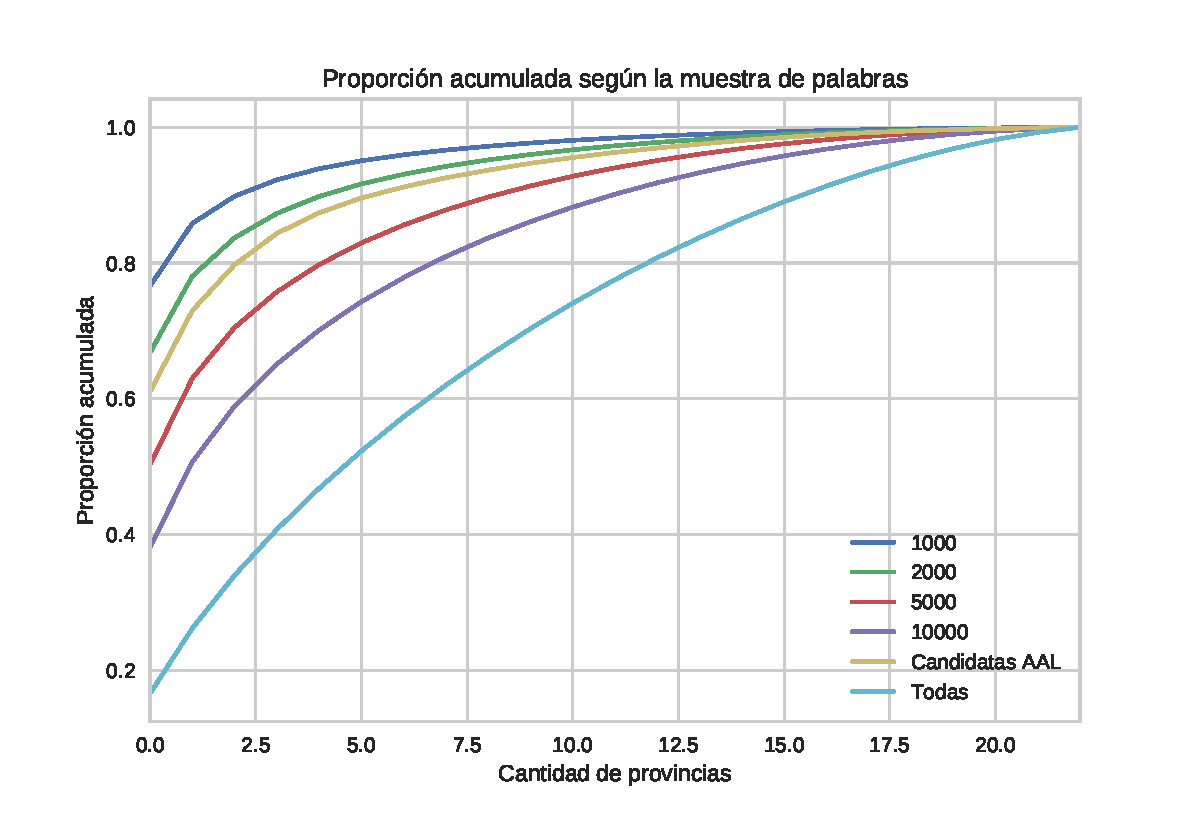
\includegraphics[width=0.44\textwidth]{images/PropAcum.pdf}
    

\end{subfigure}
~
\begin{subfigure}[b]{0.5 \textwidth}
    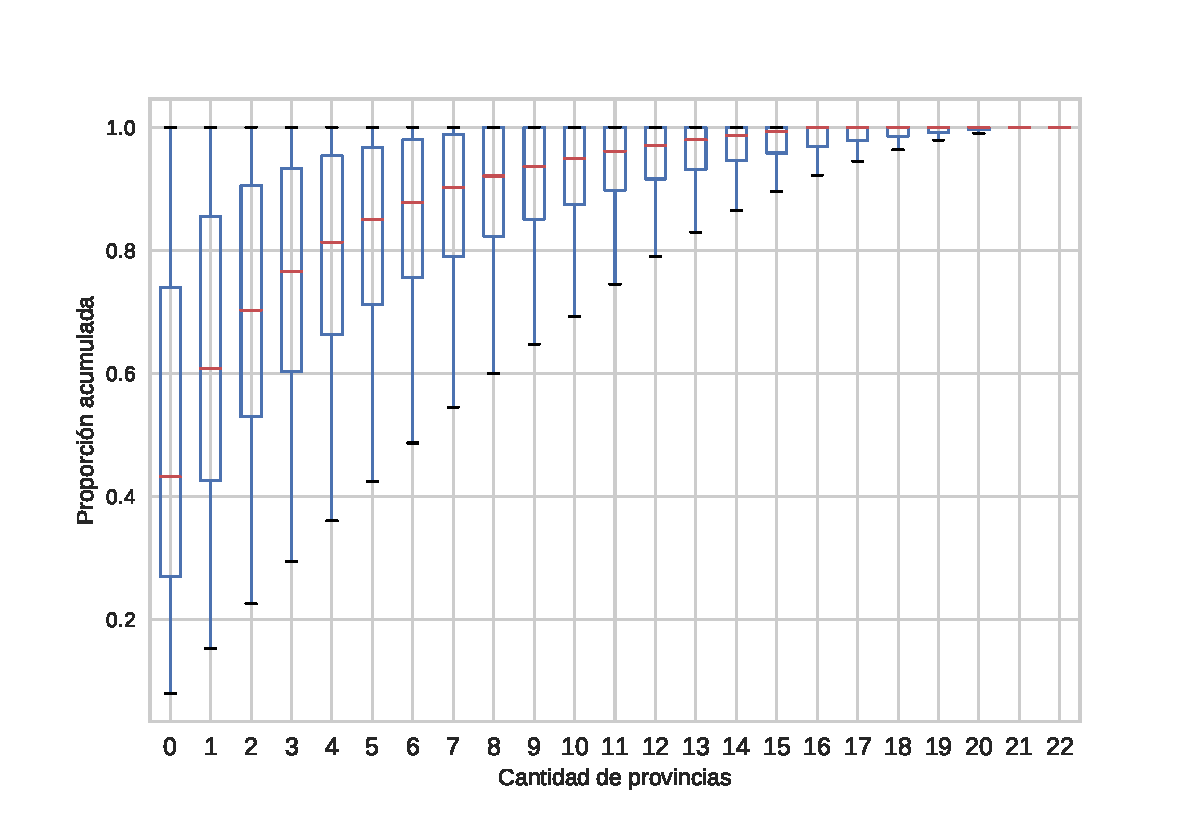
\includegraphics[width=0.44\textwidth]{images/PropAcum5000.pdf}
\end{subfigure}

\caption{Proporción de ocurrencias acumulada media según la muestra de palabras. El número de la leyenda indica la cantidad de palabras contrastivas elegidas para la muestra respectiva, siempre seleccionando las más contrastivas según la métrica. En cada curva se refleja el promedio de la proporción acumulada de una muestra variando la cantidad de provincias que forman las regiones maximales.}
%\caption{Variación de la proporción de ocurrencias acumulada a partir de la muestra con las primeras 5000 palabras con mayor valor de contrastividad.}
\label{fig:propAcum}

\end{figure}
